\chapter{Design}

As the final prototype will utilise intermixing to affect a behaviour, two different prototypes will have to created. One that is overloaded with the message (75 percent) and one that is intermixed (45 percent). The following chapter will explain how the design came to be and the decisions that affected the final design.

\section{Final design; Burger Car}

\subsection{Narration}

\subsection{Graphics}

\subsection{Environment}

\section{Usability test}
    For discerning the usability of the interactions in the design, a simple test using the SUS scale questionnaire, was conducted. The test participant were told to put the Virtual Reality headset on their head, and got one controller handed to their primary hand. The participant were observed during the test, and afterwards instructed to fill out the SUS questionnaire.
    
\subsection{Test setup}
    The setup for the Usability test (seen in \autoref{fig:usabilitySetup}), using the SUS questionnaire, where the test subject, going through the test, were positioned in front of the monitor with the HMD on. The observer seated nearby, were noting any miscellaneous usability related things.
    
\begin{figure}[H]
    \centering
    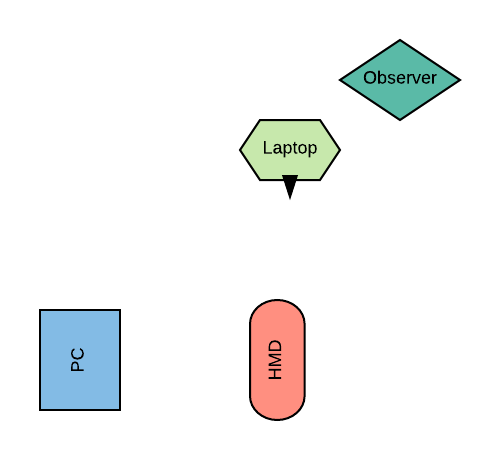
\includegraphics[width=0.6\linewidth]{figure/Design/UsabilitySetup.png}
    \caption{The setup of the usability test, with the \color{red}{HMD/User}, \color{blue}{PC}, \color{teal}{Observer}, and \color{green}{Laptop for SUS}}
    \label{fig:usabilitySetup}
\end{figure}

\subsection{Test results}
After the test participants have answered all 10 questions on the SUS questionnaire, the SUS score that values the usability of the design, is calculated using the official SUS method\cite{SUS}. For all odd numbered questions (1, 3, 5, 7, and 9,) 1 is subtracted from the score. For all even numbered questions (2, 4, 6, and 8,) the scores are subtracted from 5, this results in the all question scores being between the range of 0 and 4. These new scores are summed up and multiplied by 2.5, resulting in a number between 0 and 100\cite{SUS}. The final numbers' mean resulted in a mean of 87, which in SUS terms, means that the usability of the design is rated at excellent\cite{SUS}. All the individual calculated SUS scores and their reference points can be seen in \autoref{fig:susplot}. 

    \begin{figure}[H]
        \centering
        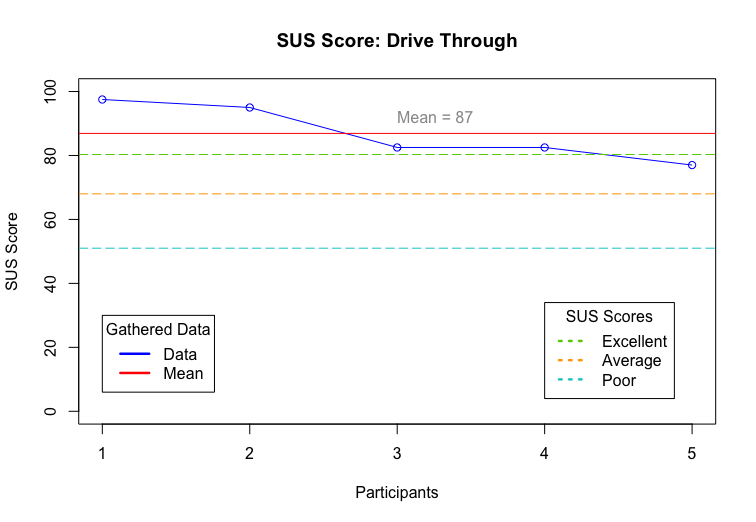
\includegraphics[width=0.8\linewidth]{figure/Design/susplot.png}
        \caption{SUS plot showing the calculated SUS score for each participant. With a total of mean of 87, the score is above the threshold that is stated to be an excellent SUS score.}
        \label{fig:susplot}
    \end{figure}

\subsection{Observations}
    During the usability test, an observer noted any usability issues that would occur. These notes correlated into the issue that $\frac{4}{5}$ test participants initially did not press the correct trigger on the Oculus touch controller when grabbing for the burger, and then being confused about how to grab the burger. Eventually $\frac{5}{5}$ users figured out that the controller had two trigger buttons, and then proceeded to expectedly grab the burger and quite naturally move it towards their mouth and eat it. This button was changed to the button that most test participants found natural to press to grab the burger. It was also noted that $\frac{5}{5}$ test participants smiled when the natural reaction to eat the burger, and outcome of eating the burger in Virtual Reality connected.
    
\section{Design summary}
